\section{Link Length Optimization}
\label{sec:link_length_optimization}
This section details the optimization of the robot's link lengths to maximize jumping performance. The optimization ensures the robot can achieve sufficient jump heights for future reinforcement learning (RL) control policy training and demonstration. A grid search approach using a simplified Simscape robot model systematically explores different link length configurations.

\subsection{Problem definition}
The link lengths and initial pose critically determine the robot's jumping capability due to the passive knee spring actuation. Link lengths constrain the possible initial poses for a given jumping angle, while the pose determines spring compression and thus available potential energy. Additionally, link lengths affect the center of mass trajectory during jumps, influencing how gravitational and ground contact forces impact the robot's movement. A grid search using a simplified Simscape model (detailed in section \ref{sec:modeling_and_simulation}) identifies optimal link lengths.

\subsection{Problem simplification}

While the robot should jump both vertically and at angles to overcome obstacles, optimizing for angled jumps presents challenges. We want to directly compare the jumping performance of different link lengths, but it is not obvious how to place the initial pose of the robot to achieve any given jumping angle using only the passive actuation of the knee springs. This is a problem for future RL control policies.

%TODO: Daniel, missing figure
To simplify the optimization, only the vertical jumping performance was considered, so that different link lengths can be compared directly. Vertical jumps are achieved across link lenghts by flipping the front legs, such that the legs are symmetric by the vertical axis, as shown in figure \ref{fig:link_length_optimization:flipped_legs}. In this configuration, the movement of the legs during the jump is symmetric and the robot center of mass remains in the horizontal center of the robot, such that any horizontal component of the jump is canceled out. Though this is not the asymmetric leg configuration the robot will use in practice, it provides an approximation for the jumping performance of a given link length configuration. The metric used to evaluate the jumping performance is the maximum height reached by the center of mass of the robot body, minus the maximum standing height reached by the center of mass of the robot body when the legs are fully extended and the paws are in contact with the ground.

The asymmetric leg configuration can also achieve vertical jumps by adjusting the angle between the hip-to-paw vector and vertical, as shown in figure \ref{fig:link_length_optimization:asymmetric_legs_vertical_jump}. However, finding or calculating the optimal offset for arbitrary link lengths is complex. We therefore simplify by placing paws directly beneath hips, except when $L2>L1$. While this produces less realistic jump heights, it greatly simplifies optimization.

For $L2>L1$ configurations, placing paws directly under hips results in near-vertical legs that slip during jumps. We prevent this by translating paws slightly inward (figure \ref{fig:link_length_optimization:symmetric_config_adjusted_paws}). This better approximates the practical asymmetric case where paws require similar translation for vertical jumps. To handle the increased opposing horizontal forces between paws in the symmetric configuration, we double the friction coefficients from 1.0/0.8 to 2.0/1.6 (static/kinetic), which further reduces slipping.

\begin{figure}[h]
    \centering
    \begin{subfigure}[b]{0.48\textwidth}
        \centering
        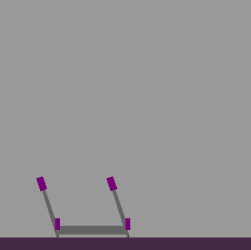
\includegraphics[width=\textwidth]{Images/link_length_optimization/unadjusted_paw_pose.png}
        \caption{Initial pose with unadjusted paws}
    \end{subfigure}
    \hfill
    \begin{subfigure}[b]{0.48\textwidth}
        \centering
        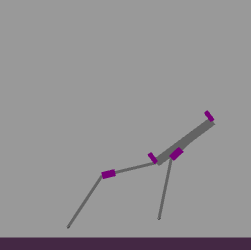
\includegraphics[width=\textwidth]{Images/link_length_optimization/unadjusted_paw_jump.png}
        \caption{Resulting angled jump}
    \end{subfigure}
    \caption{Unadjusted paw placement results in angled jump}
    \label{fig:link_length_optimization:unadjusted_jump}
\end{figure}

\begin{figure}[h]
    \centering
    \begin{subfigure}[b]{0.48\textwidth}
        \centering
        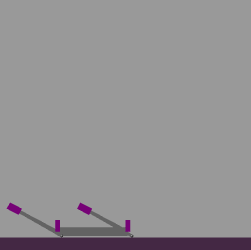
\includegraphics[width=\textwidth]{Images/link_length_optimization/adjusted_paw_pose.png}
        \caption{Initial pose with adjusted paws}
    \end{subfigure}
    \hfill
    \begin{subfigure}[b]{0.48\textwidth}
        \centering
        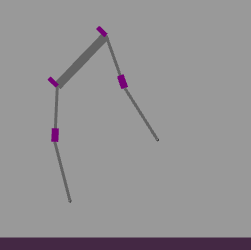
\includegraphics[width=\textwidth]{Images/link_length_optimization/adjusted_paw_jump.png}
        \caption{Resulting vertical jump}
    \end{subfigure}
    \caption{Adjusted paw placement enables vertical jump}
    \label{fig:link_length_optimization:adjusted_jump}
\end{figure}


\begin{figure}[h]
    \centering
    \begin{subfigure}[b]{0.48\textwidth}
        \centering
        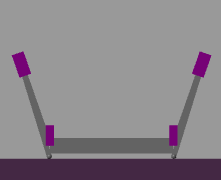
\includegraphics[width=\textwidth]{Images/link_length_optimization/symmetric_unadjusted_paws.png}
        \caption{Paws directly under hips leading to near-vertical legs}
    \end{subfigure}
    \hfill
    \begin{subfigure}[b]{0.48\textwidth}
        \centering
        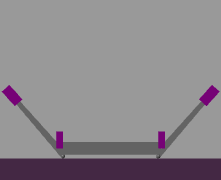
\includegraphics[width=\textwidth]{Images/link_length_optimization/symmetric_adjusted_paws.png}
        \caption{Paws translated inward to make legs more horizontal, which reduces slipping}
    \end{subfigure}
    \caption{Paw placement adjustment for $L2>L1$ configurations}
    \label{fig:link_length_optimization:symmetric_config_adjusted_paws}
\end{figure}


\begin{figure}[h]
    \centering
    \begin{subfigure}[b]{0.48\textwidth}
        \centering
        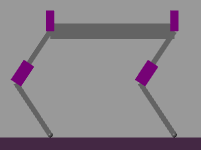
\includegraphics[width=\textwidth]{Images/link_length_optimization/asymmetric_legs.png}
        \caption{Normal asymmetric leg configuration}
    \end{subfigure}
    \hfill
    \begin{subfigure}[b]{0.48\textwidth}
        \centering
        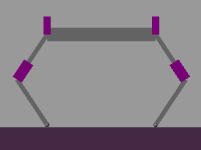
\includegraphics[width=\textwidth]{Images/link_length_optimization/symmetric_legs.png}
        \caption{Symmetric leg configuration for vertical jumping}
    \end{subfigure}
    \caption{Comparison of normal and symmetric leg configurations}
    \label{fig:link_length_optimization:flipped_legs}
\end{figure}


\subsection{Initial Pose Calculation}
For each set of link lengths, an initial pose must be calculated that satisfies several constraints:

The initial pose must satisfy four key constraints: the paws must maintain ground contact, knee angles must be maximized to store maximum spring potential energy, knees cannot penetrate the ground, and both knees bend outward rather than inward to avoid self-collision.

Due to the symmetric leg configuration, the initial pose is identical but flipped for both front and back legs, ensuring vertical jumps.

The pose calculation considers three cases based on link length ratios:

\begin{enumerate}
    \item \(L_1 = L_2\) (equal lengths)
    \item \(L_2 > L_1\) (longer lower link)
    \item \(L_1 > L_2\) (longer upper link)
\end{enumerate}

For all cases, we calculate the distance \(d\) from hip to paw. For cases $L1=L2$ and $L1>L2$, where paw is placed directly under hip, this distance is vertical from the hip. For case $L2>L1$, where paw is translated horizontally inwards towards the body, this distance is along a vector with angle 0.3 radians inwards towards the body from the vertical. This offset was found to avoid any slipping in most cases, while simultaneously making jumps in the asymmetric leg configuration more realistic. 

The distance \(d\) should be as small as possible to maximize the knee angle and thus spring load while satisfying the physical constraints of the robot and keeping the paws in contact with the ground. Inverse kinematics then determines the hip and knee angles, selecting the solution where knees bend outward. The distance \(d\) is calculated as follows:

\begin{itemize}
    \item For \(L_1 = L_2\): \(d = \epsilon\), where \(\epsilon\) is a small offset ensuring unique inverse kinematics solutions
    \item For \(L_2 > L_1\): \(d = L_2 - L_1 + \epsilon\), where \(\epsilon\) prevents vertical legs and ensures sufficient ground friction
    \item For \(L_1 > L_2\): \(d = \sqrt{L_1^2 - L_2^2}\), derived when \(L_2\) is horizontal (maximizing spring load) and forms a right triangle with \(L_1\) and the hip-to-paw vector
\end{itemize}

\begin{figure}[h]
    \centering
    \begin{subfigure}[b]{0.32\textwidth}
        \centering
        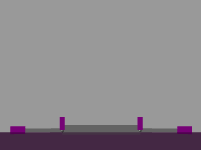
\includegraphics[width=\textwidth]{Images/link_length_optimization/equal_len_pose.png}
        \caption{Equal lengths (L1=10cm, L2=10cm)}
    \end{subfigure}
    \hfill
    \begin{subfigure}[b]{0.32\textwidth}
        \centering
        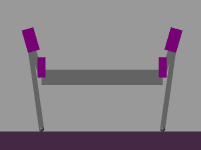
\includegraphics[width=\textwidth]{Images/link_length_optimization/longer_L2_pose.png}
        \caption{Longer L2 (L1=15cm, L2=10cm)}
    \end{subfigure}
    \hfill
    \begin{subfigure}[b]{0.32\textwidth}
        \centering
        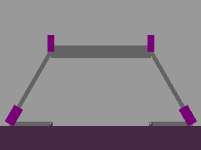
\includegraphics[width=\textwidth]{Images/link_length_optimization/longer_L1_pose.png}
        \caption{Longer L1 (L1=15cm, L2=10cm)}
    \end{subfigure}
    \caption{Initial poses for different link length ratios}
    \label{fig:link_length_optimization:initial_poses}
\end{figure}



\subsection{Grid Search}
The grid search varies two parameters: L2/L1 ratio, and total leg length L1+L2, focusing around $L2/L1\approx1$ where preliminary tests indicated generally better performance. Simscape updates the robot mass for each parameter set. Tests were run in both Earth (9.81 $m/s^2$) and Mars (3.72 $m/s^2$) gravity, with results in figure \ref{fig:results:grid_search_results}.


